\documentclass[12pt]{article} 
\usepackage{enumerate,geometry,fancyheadings,float,shortcuts,amsmath,lastpage,ifpdf,paunits,multicol}
\geometry{letterpaper,top=50pt,hmargin={20mm,20mm},headheight=15pt} 

\ifpdf
    \usepackage[pdftex]{graphicx} 
    \usepackage{hyperref}    \pdfcompresslevel=0
    \DeclareGraphicsExtensions{.pdf,.jpg,.mps,.png}
\else
    \usepackage{hyperref}
    \usepackage[dvips]{graphicx}
    \DeclareGraphicsRule{.eps.gz}{eps}{.eps.bb}{`gzip -d #1}
    \DeclareGraphicsExtensions{.eps,.eps.gz}
\fi

\pagestyle{fancy} 
\lhead{Name:}
\chead{A405 2024 final}
\rhead{page~\thepage/\pageref{LastPage}}
\lfoot{}
\cfoot{}
\rfoot{}
\begin{document}

Instructions -- Do all questions (note weights) showing all you work.  Don't forget to put your name on your tephigram.

\begin{enumerate}

\item (10)   Cooling:  A cloud at a pressure of 600 hPa and temperature of 5 deg C has 12 g/kg of total water.  Suppose it cools by 10 K and rains so that at -5 deg C it has 1 g/kg of liquid water remaining.  Find

  \begin{itemize}
  \item[1.] The total precipitated water, in g/kg

  \item[2.] The total change in moist static energy $h_m$ in J/kg
  \item[3.] The lifting condensation level before and after the cooling, in hPa
    
  \end{itemize}
  
\item (8) Taylor series

  Recall that buoyancy for a parcel is defined

  \begin{equation}
    \label{eq:buoy}
  buoyancy = g \frac{\rho_{env} - \rho_{parcel}}{\rho_{env}} \approx g \frac{T_{vparcel} - T_{venv}}{T_{venv}}
\end{equation}


\begin{itemize}
\item[1.] Use a Taylor series expansion to derive \eqref{eq:buoy} showing the second order terms you drop.  (Hint, expand in the small parameter $\Delta T_v/T_{venv}$, where $\Delta T_v = T_{vparcel} - T_{venv}$)

\item[2.] Suppose a parcel at $T_v$=281 K maintains a 1 degree temperature difference over an environment at $T_{venv}$=280 K for an extended period of time.  How many minutes would it take for the parcel to reach a velocity of 10 m/s?


\end{itemize}

  
\item (8) Suppose you know that cloud drops have a size distribution given
  by 
  \begin{equation}
    \label{marshall}
    N(r)=N_0 \exp (- \chi r)
  \end{equation}
\noindent
where $N(r)$ ($\mathrm m^{-3}$) is the number of drops per unit volume with radius $>
r$ (for radii $50\ \mathrm{\mu m} < r < 200\ \mathrm{\mu m}$ ) and $N_0$
and $\chi$ are constants and $r$ is in $\mu m$.  Suppose also that the drop fall speed
$v(r)\ (\mathrm{m\,s^{-1}})$ 
depends on linearly on radius:
\begin{equation}
  \label{fallspeed}
  v(r)=Jr
\end{equation}
where $J= 6000\ s^{-1}$ and now $r$ is in meters.

Derive equations (including unit conversions if necessary) for:

\begin{enumerate}
\item The number density $n(D)$ ($m^{-3}\,\mu m^{-1}$)
\item The liquid water content ($\mathrm{kg\,m^{-3}}$)
\item The precipitation rate ($\mathrm{mm\,hr^{-1}}$)
\end{enumerate}


\item (10) Collision/coalescence

   Derive with the help of a sketch the simple model of the growth of rain drops represented by
   equation (\ref{eq:collec}), defining all your symbols.  If the fall speed is given by $J= 6000r \ m\,s^{-1}$ as in (\ref{eq:collec}), roughly how long would it take a 50 \mum radius drop to double to 100 \mum radius, given $w_l = 0.3\ g\,m^{-3}$?  What processes need to be added to
    (\ref{eq:collec}) to make the description of rain formation more
    accurate? Explain.


\item (11) K\"ohler curve

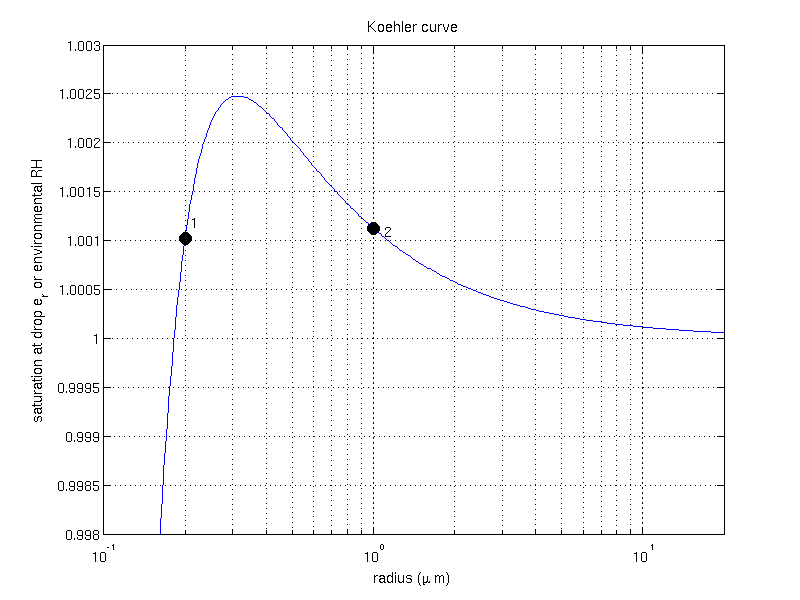
\includegraphics[width=\textwidth]{m18.png}

The figure shows two droplets with radii of 0.2 \mum and
1 \mum at a environmental relative humidity of about 1.001.

\begin{enumerate}
\item (3) Both droplets lie on a curved line called the Koehler curve.  What
do points on this line represent?  i.e.  what is it that all points lying on
this line have in common?


\item (4) Suppose the relative humidity increases from 1.001 to 1.002.  Describe
qualitatively what happens to the two drops.



\item (4) Quantitatively, what is the initial evaporation/growth rate of droplet
2 in microns/second, assuming a RH of 1.002, temperature T=280, esat(T)=10 hPa.

\end{enumerate}


\item (10) Adiabatic ascent

  Suppose someone asks you to provide the temperature, pressure, water vapor mixing ratio and liquid water mixing ratio as a function of height for surface air at press= 1000 hPa, temperature T and relative humidity RH as it ascends adiabatically through the atmosphere.  Using pseudo code sketch out a python script that would do this assuming a hydrostatic balance.  Assume you can use odeint and the rootfinder as needed.   Note:  1) the equations you would need to solve and 2) how you would solve them.


\end{enumerate}

\newpage

\begin{center}
  \textbf{Equation sheet}
\end{center}

\begin{multicols}{2}

  \begin{equation}
\label{eq:first}
du = q\,dt - w\,dt = q\,dt - p\,d\alpha
  \end{equation}

\begin{equation}
e = \rho_v\, R_v\, T
\end{equation}

\begin{equation}
p = \rho\, R_d\, T_v
\label{eq:eqstate}
\end{equation}


\begin{equation}
w \,dt = p\,d\alpha
\end{equation}

\begin{equation}
h = u + p \,\alpha
\end{equation}

\begin{equation}
  \label{eq:tv}
  T_v = T(1 + 0.608 r_v - r_l)
\end{equation}

\begin{equation}
  \label{eq:wv}
  r_{vs} = \rho_s/\rho_d = \epsilon \frac{e_s}{p - e_s}
\end{equation}

\begin{equation}
dh = c_{px}\, dT\ \mathrm(dry\ air\ or\ liquid)
\end{equation}

\begin{equation}
dh = c_p\, dT\ + l_v\,dr_v\ \mathrm(air/water\ mixture)
\label{eq:dhdef}
\end{equation}


\begin{equation}
dh = T\,d\phi + \alpha\,dp\ \mathrm(reversible)
\label{eq:reversible}
\end{equation}

\begin{equation}
d\phi = c_p \frac{d\theta}{\theta} = c_p \frac{dT}{T} - R_d \frac{dp}{p}
\label{eq:thetadef}
\end{equation}

\begin{equation}
  \label{eq:dphi}
  d\phi \geq \frac{q\,dt}{T}
\end{equation}

\begin{equation}
l_v = h_v - h_l
\end{equation}


\begin{equation}
dp = - \rho\,g\,dz
\label{eq:hydro}
\end{equation}


\begin{equation}
\label{eq:moist}
  dh_m = c_p\,dT + l_v\,dr_v + g\,dz
\end{equation}

\begin{equation}
\label{eq:thetaes}
  d\phi = c_p \frac{d\theta_{es}}{\theta_{es}} = c_p \frac{d\theta}{\theta} + \frac{l_v\,dr_s}{T}
\end{equation}

\begin{equation}
  d\phi = c_p \frac{d\theta_l}{\theta_l} = c_p \frac{d\theta}{\theta} - \frac{l_v\,dr_l}{T}
\end{equation}


\begin{equation}
  \label{eq:wdiff}
  d r_v = \frac{r_v}{p-e} \left ( \frac{p}{e} de - dp \right )
\end{equation}

\begin{eqnarray}
  \label{eq:taylor}
  f(x)  &=& f(x_0) + f^\prime(x_0)(x - x_0) \nonumber\\ 
        &+&  \frac{f^{\prime\prime}(x_0)}{2}(x-x_0)^2 +  \ldots
\end{eqnarray}

\begin{gather}
\label{eq:cc}
  l_v = T (\phi_v^* - \phi_l)
\end{gather}

\begin{gather}
  \frac{de_s }{dT} = \frac{l_v e_s}{R_v T^2} 
\end{gather}


\begin{subequations}
  \begin{eqnarray}
  h_l = c_l (T - T_p) \\
 h_v = l_{v0} + c_{pv} ( T - T_p) \\
\phi_d = c_{pd} \ln T - R_d \ln p_d \label{eq:dryentrop}\\
 \phi_l = c_l \ln \frac{T }{T_p}  \\
\phi_v = c_{pv} \ln \frac{T }{T_p} - R_v \ln \frac{e }{e_{s0}} + \frac{l_{v0} }{T_p}  
\label{eq:sdef}
  \end{eqnarray}
\end{subequations}


  \begin{equation}
  g = u + p\alpha - T\phi = h - T\phi
\label{eq:gdef}
  \end{equation}

  \begin{equation}
    \label{eq:dg}
    dg \leq -\phi dT + \alpha dp
  \end{equation}


  \begin{equation}
    \label{eq:G}
    G = m_v g_v + m_l g_l + 4 \pi \sigma r^2
  \end{equation}

  \begin{equation}
    \label{eq:newint}
    \int_{a_w e_s}^e  d(g_l - g_v) \approx  - R_v T\ln \left (
      \frac{S}{a_w} \right )
  \end{equation}



\begin{multline}
  \label{equil}
  e_{r} = e_s(T)(n_w/(n_w + n_s))\exp(a/r) \\
  = e_s(T)(1 + \frac{a}{r} - \frac{b}{r^3})
\end{multline}

\begin{equation}
  \label{eq:sscrit}
  s_{crit}= 1 + \left ( \frac{4 a^3}{27 b} \right )^{1/2}
\end{equation}

\begin{equation}
  \label{eq:rcrit}
  r_{crit} = \left ( \frac{3b}{a} \right )^{1/2}
\end{equation}

\begin{gather}
  \label{eq:2ndb}
  c_p \frac{d\theta_e^\prime}{\theta_e^\prime} = 
          \frac{dm}{m} \frac{\Delta h_m}{T^\prime} = \frac{dm}{m} \Delta s \nonumber\\
   = c_p \frac{dm}{m} \Delta \ln \theta_e    
\end{gather}

\begin{equation}
  \label{eq:plume}
  \frac{1}{m} \frac{dm}{dt} = \lambda
\end{equation}

\begin{equation}
  \label{eq:water}
  \frac{dr_T^\prime}{dz} = (r_T - r_T^\prime) \hat{\lambda}
\end{equation}

\begin{equation}
  \label{eq:collec}
  \frac{dM}{dt} = \pi R^2 E_c (V(R) - V(r)) r_l
\end{equation}
where V(r) $\approx$ 0 and V(R) $\approx$ JR (with J=6000 $s^{-1}, R in \un{m}$)

\begin{equation}
  \label{eq:dropgrow}
  \frac{dm}{dt} = 4 \pi r D (\rho_{v \infty} - \rho_{v r})
\end{equation}

\begin{gather}
  \frac{ dr}{dt} = \frac{ 1}{r} \frac{ D \rho_{v \infty}}{\rho_l e_\infty}  [e_\infty - e_{r}]
\label{eq:dropgrowr}
\end{gather}


\begin{gather}
      N(D^\prime)= \int_{D^\prime}^\infty n(D)dD
      \label{eq:cumulative}
\end{gather}

\label{constants}
\begin{tabular}{ll}
$a$ & $\frac{2 \sigma}{\rho_l R_v T}$  \\
$b$  &  $\frac{i m M_w}{(4/3)M_s \pi\rho}$ \\ 
$\sigma$ & 0.075 \un{J\,m^{-2}}\\
$\rho_l$ & 1000  $\un{kg\,m^{-3}}$ \\
$c_{pd}$ & 1006\ \un{J\,kg^{-1}\,K^{-1}}\\
$c_{vd}$ & 719\ \un{J\,kg^{-1}\,K^{-1}}\\
$c_{pv}$ & 1870\ \un{J\,kg^{-1}\,K^{-1}}\\
$c_{vv}$ & 1408 \un{J\,kg^{-1}\,K^{-1}}\\
$c_l$    & 4190\ \un{J\,kg^{-1}\,K^{-1}}\\
$D$      & 2.36 $\times 10^{-5}$ \un{m^2\,s^{-1}}\\
$R_d$    & 287\ \un{J\,kg^{-1}\,K^{-1}}\\
$R_v$    & 461\ \un{J\,kg^{-1}\,K^{-1}}\\
$k$      & 1.381 $\times 10^{-23}$\ \un{J\,K^{-1}\,molecule^{-1}}\\
$l_{v0}$    & 2.501 $\times 10^6 $\ \un{J\,kg}\mbox{ at 0 deg C}
\end{tabular}

\end{multicols}


\end{document}


%%% Local Variables:
%%% mode: latex
%%% TeX-master: t
%%% End:
